\documentclass[30pt,twocolumn,letterpaper]{article}
\usepackage{cvpr}
\usepackage{times}
\usepackage{booktabs}
\usepackage{epsfig}
\usepackage{graphicx}
\usepackage{amsmath}
\usepackage{amssymb}
\cvprfinalcopy
\def\cvprPaperID{****}
\def\httilde{\mbox{\tt\raisebox{-.5ex}{\symbol{126}}}}
\usepackage{graphicx}
\usepackage{indentfirst}
\setlength{\parindent}{2em}
\usepackage{cite}
\usepackage[colorlinks,linkcolor=red,anchorcolor=blue,citecolor=green,backref=page]{hyperref}
\author{Qilei Zhang}
\date{Jun 2 2018}
\title{Stochastic resonance in spatially extended systems}
\begin{document}
\maketitle
\begin{abstract}
   So far we mainly investigated stochastic resonance in systems with only one degree of freedom, such as a particle moving in a potential under the influence of an external driving force and noise.
\end{abstract}
\section{Introduction}
In this section we describe how stochastic resonance manifests itself in spatially extended systems such as a string moving in a bistable potential under the influence of noise and external forcing, or in a two-dimensional medium forming spatiotemporal patterns in the presence of noise\cite{Carroll1993Stochastic}.
\begin{figure}[htbp]
\small
\centering
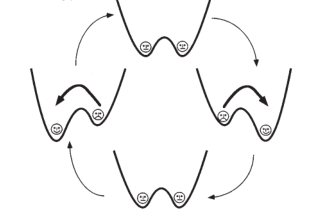
\includegraphics[width=20em]{000.png}
\caption{spatially extended systems}
\label{fig:lable}
\end{figure}
\section{Global synchronization of a bistable string}
In this section, we consider a one-dimensional bistable medium in the presence of noise and isotropic periodic forcing. A more refined analysis of stochastic resonance in a modulated string has been derived recently by Marchesoni, Gammaitoni, and Bulsara within the framework of the theory of thermal nucleation in onedimensional chains\cite{Neiman1994Stochastic}. \\
\begin{equation}
r_n=\frac{1}{T}\int_0^T r(t)exp(-inwt)dt
\end{equation}
\section{Spatiotemporal stochastic resonance in excitable media}
Pattern formation in excitable media is an important paradigm with many applications in biology and medicine such as contraction waves in cardiac muscle, slime mold aggregation patterns, and cortical depression waves, to name only a few. While most theoretical and experimental work on excitable media focuses on the propagation of spiral waves, the role of fluctuations for pattern selection and propagation has been studied only recently by using a stochastic cellular model\cite{Rallabandi2010Magnetic}.
{\small
\bibliographystyle{ieee}
\bibliography{1}
}
\end{document}
